%%\documentclass[sigconf, review=true]{acmart}
\documentclass{aircc}

\usepackage{graphicx}
\usepackage{wrapfig}



\title{Dynamic aspect ratio}
%% \acmConference{MMSYS}{2022}{Ireland}

\author{Njål Borch $^1$ and Ingar Arntzen $^2$}
\affiliation{NORCE Norwegian Research Institute \\ $^1$\email{njbo@norceresearch.no} \\ $^2$\email{inar@norceresearch.no}}

\bibliographystyle{plain}


%%\author{Ingar Arntzen}
%%\affiliation{NORCE \\ \email{inar@norceresearch.no}}

% header and footer (this would be nicer to put into cls file)
\fancyhf{}
%%\chead{\xsmall{SPPR 2022}}
\rfoot{\xsmall{\thepage}}



\begin{document}
\maketitle
\pagestyle{fancy}



\begin{keywords}
Dynamic aspect ratio, Focus track, Multi-device, client side, AI analysis
\end{keywords}


%%\begin{acks}
%%This work is financed by the
%%\grantsponsor{mediafutures}{MediaFutures research center in Bergen, Norway}{mediafutures.no}
%%\end{acks}

 
\begin{abstract}

%% Just say that there are many aspect ratios in use today.

Media is to a large extent consumed on devices that have non-standard aspect
ratios, both physically or while rendering content. 

For example, social media platforms often favour 1:1 ratios, TVs 16:9, iPad
tablets 4:3 or 3:4, most Androids 16:9 or 9:16, PCs 16:9 or 16:10 and web
pages tend to use responsive design and can therefore have almost any aspect
ratio

In order to ensure good experiences, it is often therefore necessary to create
multiple versions of content, where the content is cropped to a more suitable
format. Creating multiple encoded version of the content is a static solution
though, and there are good reasons for solving this dynamically on the client
side. 

In this paper we make the case for a client side dynamic aspect ratio
solution, present work on implementation and experimentation, and finally
provide some insights into how such a system could be implemented and
provided in real world systems. Our solution was tested on a few different
pieces of content from NRK, both drama series and typical TV debates.

\end{abstract}


\section{Introduction}\label{introduction}

The iPhone arrived with sensors allowing it to rotate the screen dynamically
in response to how it was held, and responsive web pages allow this also for
web content. This has led to a highly dynamic and arbitrary available screen
realestate for online video content. We also observe that a large fraction of
users hold their phones in portrait mode when watching video content, as
shown in figure \ref{scientiamobile}. Only larger tablets are mostly held in
landscape mode. A 16:9 aspect ratio video file displays particularly poorly
on a small 9:16 screen. In extreme cases, horizontal videos, typically user
provided content, is re-created as 16:9 content by a video streaming service,
then presented to the user on a 9:16 screen. This makes the actual content
only 10 percent of the natural display size. Even if watched in landscape
mode, the content is still only 31 percent of the available screen estate. 

\begin{figure}
  \begin{center}
    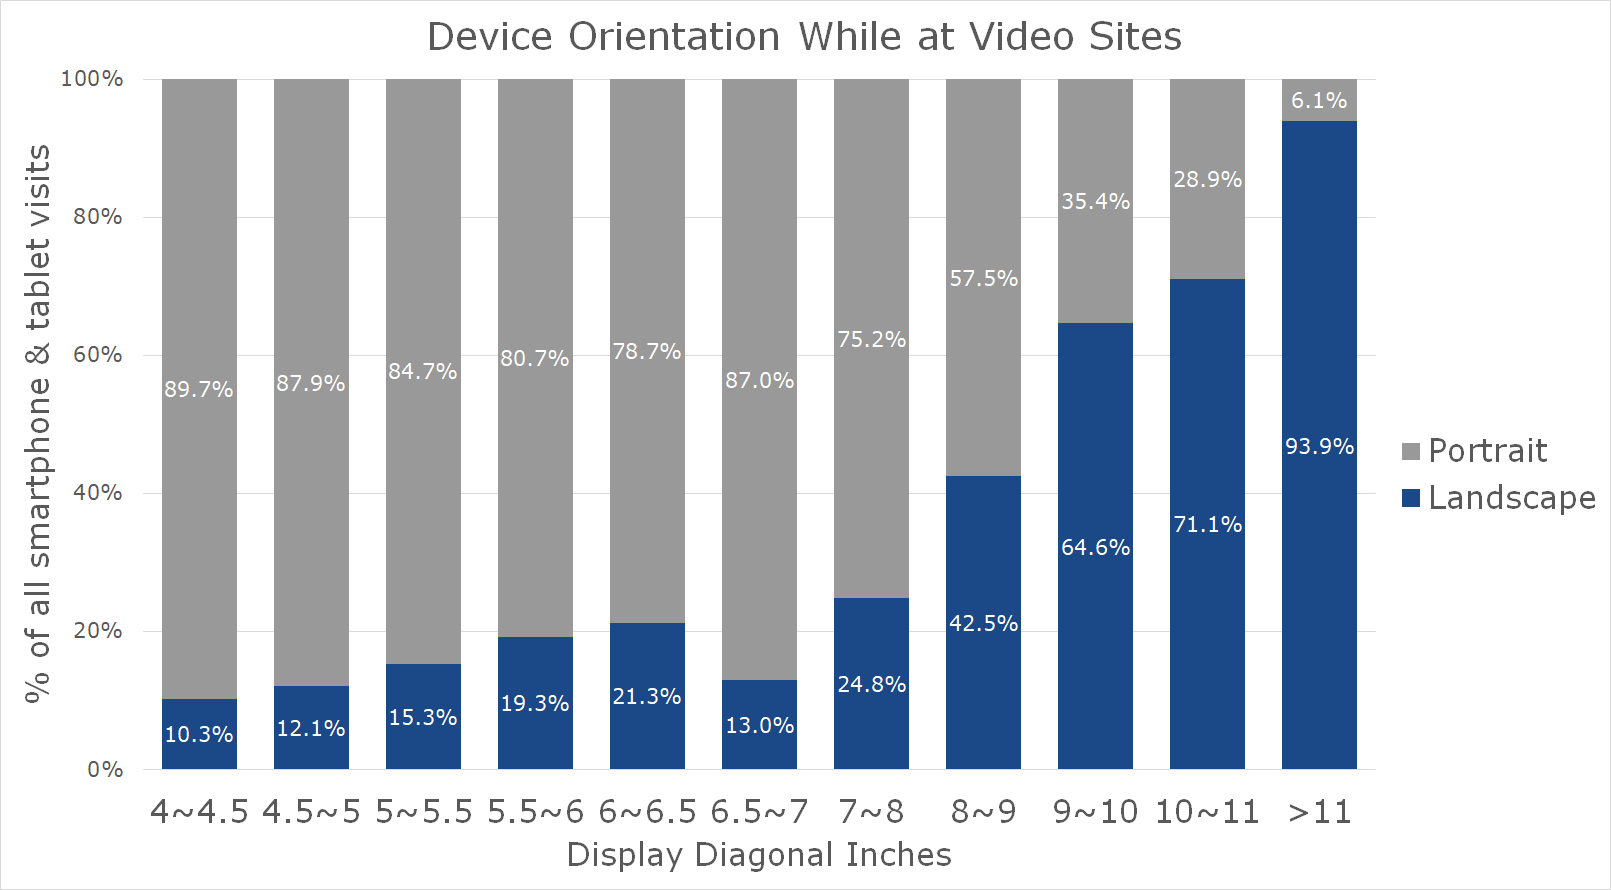
\includegraphics[width=0.7\columnwidth]
     {device-orientation-by-diagonal-size-video-sites-v2.png}
  \end{center}
  \caption{Orientation on video sites, ScientiaMobile 2019.}
  %%\Description{Most video content is consumed in portait mode on devices with
  %% a screen size smaller than 9 inches.}
  \label{scientiamobile}
\end{figure}

At the same time, a large amount of video is watched on mobile phones.
According to \cite{hootsuite}, 70\% of YouTube traffic is on mobile devices,
which translates to a staggering 700 million hours of video each day being
watched on mobile devices on YouTube alone (Jan 2021). Being able to provide
better, more immersive services on mobiles will continue to be of high
importance. Dynamically adapting to any display ratio can provide substatial
added value.

In addition there is also a case to be made from a cognitive angle. A
production for large screens might easily include a lot of scenery to provide
ambience for a scene. For smaller displays, this means that very little space
is used to actually present the driving parts of the content. Recognizing
facial expressions on a face that is less than a centimeter squared puts a
substantial demand on eye sight and concentration. In such scenarios,
watching a cropped video in portrait mode will allow faces to become much
larger and therefore easier to understand as can be observed in figure \ref
{croppings}.

\begin{figure*}
  \begin{center}
    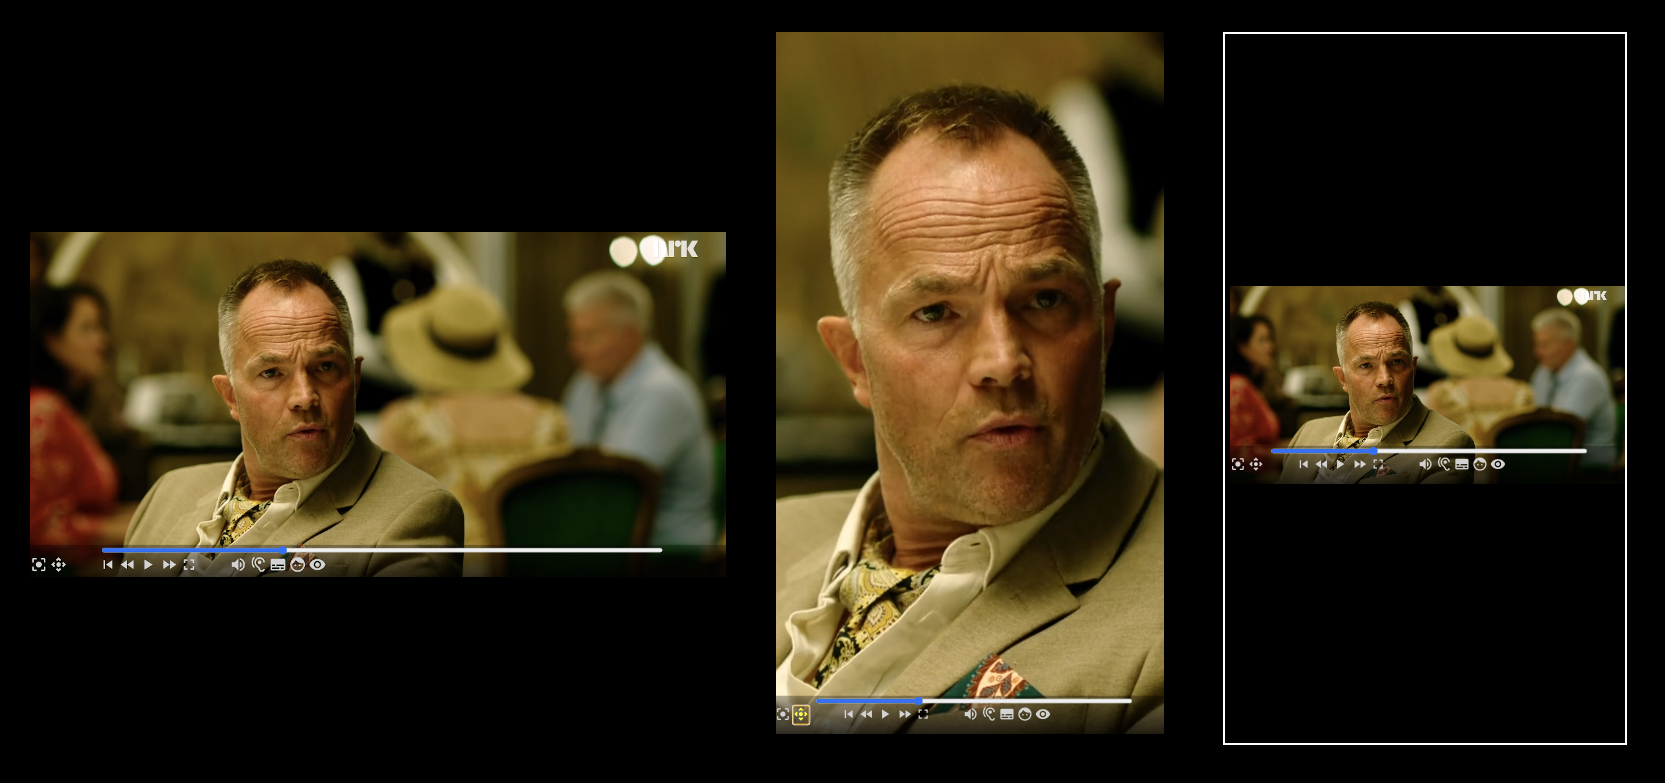
\includegraphics[width=0.9\textwidth]{DAR_vs_letterbox.png}
  \end{center}
  \caption{16:9 landscape, 9:16 dynamic crop and 9:16 letterboxed, same size screen.}
  \label{croppings}
  %%\Description{Different renderings of a video on the same size device,
  %% dynamic crop shows face very clearly.}
\end{figure*}

In this paper we discuss using a dynamic client side cropping of video content
based on a focus track providing the focus point of the experience. This is
done the different data is transferred to the client, possibly individually,
and then synthesized into the final presentation by the client itself. We
also present our work on automatic production of focus tracks for a few
different types of production, as well as prelimiary findings on the final
output.

%%\section{Background}
\section{Related work}

Altering aspect ratios is not a new concept and was prevalent in adapting
films to 4:3 TV sets. There are three fundamental ways to transform the
aspect ratio. The first is to pad the content with black areas, trading
screen real estate for an accurate representation of all video pixels
(letter-boxing). The second is to do a fixed crop for the whole asset
(typically the center). This can lead to very unpleasing visuals, as images
composition is often placed either according to the golden ratio or the "rule
of thirds", avoiding center focus. A center crop will thus often cut the item
in focus. The third option is to create positioning data for the focus point
or area for each frame or scene, which in this paper will be referred to as
a "focus track". A crop is then created using this focus track, in effect,
cutting away the least imporant bits of the content. Approaches like
streching or compressing the content are not discussed in this paper as they
distort the image.

Focus tracks can be made manually, the process can be automated or a hybrid
process combining automated with manual quality control can be used. Most
focus tracks are currently used directly to crop images as the focus is being
determined, and these tracks are therefore internal in the tools and often
not persisted.

Manual focus tracks, or direct cropping for physical mediums, is a labour
intensive task. Automating the process has received ample research, and as
the number of possible aspect ratios have increased, so has the importance of
this area. In \cite{liu2006video} a process using image analysis was used to
do "pan and scan", retargeting videos for other aspect ratios. A number of
commercial and experimental tools and services now exist to automate the
process of cropping video to a number of aspect ratios \cite
{adobe_premiere,mediapipe,kamua}. The MediaPipe\cite{mediapipe} project from
Google provides a service called "AutoFlip", which uses OpenCV to convert one
video into a number of predefined aspect ratios, using various object and
other detections to understand the video frames. In our experiments, we have
indeed used the MediaPipe library as one method of generating focus tracks.

Common to these existing solutions, the focus track is internal and is used to
apply cropping as a part of the postproduction phase. This leads to multiple
video encodings being stored and distributed at different aspect ratios as
separate assets. As multi-bitrate videos like MPEG DASH or HLS are highly
popular to ensure good end user experiences also on slower networks, each
aspect ratio asset will have multiple encodings as well. With 4 different bit
rates and 5 aspect ratios (16:9, 4:3, 1:1, 3:4 and 9:16) a total of 20
versions of every single asset is necessary as opposed to 4 with client side
cropping. Even worse, if a sign language interpreter is embedded in the
video, the number of assets would now be 40, while client side focus track
and video overlay would limit this to just 5.

Solutions using fixed cameras and AI processing to provide low-cost, automated
productions is also becoming available\cite{ai_sports}. A set of cameras are
typically stiched together to provide a very high resolution image of the
entire play field. An AI specially trained for a particular sport will then
determine the area of interest at any given time, and an output video is then
cropped from the main, high resolution input. The end result can be quite
similar to basic coverage using a single camera point with a human operator.
In such cases, a focus track is created by the AI, and is directly used to
crop the video. If the focus track was further exported, the client side
playback could further crop the video to a suitable aspect ratio while
retaining the full power of the specially trained AI. Providing focus tracks
with information about overlaid graphics could also be highly useful in order
to ensure that the graphics are visible, for example in debates.

Even more advanced systems exist, adding support for 360 degree video with 3
degrees of freedom (pitch, yaw, roll)\cite{8712670}. Such systems let users
look around using for example VR headsets. In this case, focus tracks could
provide users with a traditional lean-back experience or even some high level
choices, e.g. select team. With immersive video\cite
{yeung2020delivering} full 6 degrees of freedom is possible (x, y, z as well
as pitch, yaw, roll). In this case, focus tracks could provide lean back
presets based on for example a favourite player, team, front-row or even
production style. Being able to provide both lean forward and lean backwards
experiences based on the same media assets would open for vastly more
flexible offerings without adding additional assets, and open for many new
and innovative media experiences for a much larger number of users. 

Object based media (OBM) pioneered by the BBC provides a flexible object based
model for media, where media can both be regarded as layers and as content
segments. A dependency graph between objects allows for dynamically altering
the length of a piece of content while retaining the narrative, and layering
allows cusomized rendering for particular clients. Adoption of OBM has been
limited by a more complex production phase, and work is being done to address
this \cite{8352916}. OBM does however not provide focus tracks as such,
making it necessary for multiple assets to be provided in order to for
example alter the aspect ratio of video without risking loosing important
parts of the picture. Adding focus tracks to OBM would allow even further
customizability, ensuring that also the video data can be adapted and placed
correctly as well as ensuring that graphics are not overlaid important
areas.

Another example of client side synthesizing can be found in \cite
{JIT_video}. Live production of object based media has been shown possible,
with a focus on controlling and customizing overlay graphics while also
allowing users to select video feed for additional angles\cite
{10.1145/3209280.3209528}. These solutions do however not provide
adaptability of the video itself, and would as such benefit by adding dynamic
aspect ratio to the descriptive timeline. It would then be possible to
exploit the available screen realestate even better, pairing it with
graphics, ensuring that graphics are not overlaid important parts of the
picture etc.

A different use case where a flexible aspect ratio would be useful is when
adding a sign language interpreter. To avoid the interpreter being in the
way, a typical approach is to make the main content smaller, move it to the
top left and add a visually pleasing border. This does however reduce the
screen real estate for the video substantially. With a focus track the
interpreter can be overlaid on top of the main content and shifting the main
content to the left (with a black border on the right) if the interpreter
would otherwise overlay the focus point. This allows a larger portion of the
screen to be used for the main content while ensuring all important aspects
are visible.

Similarly, a portrait mode display including a sign language interpreter or
subtitles, will ensure that the most important area of the screen is visible
in the immediate vicinity of the user's eyes. This will limit necessary eye
movements, and at the same time limit the amount of distractions. It has also
been shown that having both text and the video content visible improves
understanding \cite{eyetracking}. Allowing text or other accessibility
features to be combined with a zoomed in video could provide users with
particular needs increased understanding of the content.


\section{Approach}

We see a number of different solutions to create focus tracks, even if they
are implicit and not persisted. Combining the wish for multiple aspect ratios
with adaptive streaming solutions means a substantial growth in the number of
files to distribute, and switching between aspect ratios is not easy.

To provide a more flexible, cheap and extendible solution, we suggest creating
explicit focus tracks that can be transferred to the client as a separate
data track. The client can then ensure that the video is cropped according to
the device capabilities and user preferences. By moving this responsibility
to the client, it is possible to use existing video assets for any aspect
ratio. Better placement of graphics also becomes possible, as clients will
know where the focus of the viewer is likely to be. As aspect ratio becomes
dynamic, relative placement (e.g. "lower right") might be in a very different
place from the video asset point of view (like "bottom center"), making it
more likely to be in conflict with other visuals. 

Our goal is to demonstrate that client side video cropping is feasible in
typical web browsers, producing a pleasing user experience. This means that
cropping needs to be frame accurate to avoid flickering effects, and that
changing aspect ratios (e.g. rotating devices) is smooth and natural.
Secondly, we want to demonstrate that such an approach does not require
changes to video formats or production flows, but can be added as a separate
process and data track. This would allow client side dynamic aspect ratio to
be added to existing systems without changes to the existing work flows, data
formats or distribution mechanisms.

In the next section, we describe our implementation of a video player than can
process a separately delivered focus track, allowing any aspect ratio. We
will then test the player with both manual and automated focus tracks to gain
experience with this approach.

%% Hva er egentlig problemstillinga? Hva prøver vi å løse?
%% Identifisert focus tracks som viktig, 
%% Goal?
%% Late binding stuff?
%% Present a plan for the implementation, the motivation, etc. 
%% Demonstrate feasibility of client side cropping, benefits of regarding the focus track as an independent resource as opposed to re-encoding, validate with both manual and automatically generated focus tracks.

\section{Implementation}

We have created a web based player that supports client side cropping
according to a given focus track. We call this dynamic aspect ratio. The
focus track can be static or dynamic and the video asset used can be any
format supported by the HTML5 video tag. The player can either show the whole
video with black borders to fill the screen, or a "zoom" button will fill the
available screen real estate using the focus track. This is done by resizing
the video to fill the available space and adjust the positioning of the video
to ensure that the focus point is still visible. Transitioning between two
positions can be either instant, which is more suitable for scene
changes/I-frame synchronized changes, or animated using a CSS "ease"
animation to provide a smooth pan movement. A manifest is created for each
resource, providing URLs to both audiovisual assets, focus track, subtitles
and other resources, as well as options for visualization if the default
values are not suitable for that partucular content.

The focus track itself provides a set of positions with a start and end time
relative to the video asset timeline, an (x,y) position and optionally also
an "animate" tag to force either animation or immediate crop change. The
player can also "auto-animate" the transitions. It does this by ignoring very
small changes, allowing frame-by-frame analysis to produce somewhat noisy
focus tracks while still producing a calm and steady output. Larger panning
movements that will look hasty will be done immediately, giving an experience
closer to changing camera angle.

As well as the dynamic aspect ratio using focus tracks, the player can also
overlay an alpha channel video of a sign language interpreter. This is kept
at the lower right, moving the video somewhat to the left if the focus point
would otherwise be covered by the overlay. There are many other uses of the
focus track as well, which have not been analyzed in this paper.

The focus tracks are kept separate from the video instead of embedded within
the container, both ensuring that the solution works for existing media
assets and that focus tracks can be produced and transferred independently of
the media distribution platform. This ensures that focus tracks can be added
to existing solutions without altering work flows or media handling.

Timing Objects \cite{Arntzen2018,timingobject} are used in combination with
sequencers \cite{sequencer} to ensure that the positioning data is tightly
sychronized with video playback. This is very important, as re-positioning
the video on the wrong frame on scene shifts is highly detectable and creates
full-screen flickering that detracts substantially from the user experience.


\section{Producing focus tracks}

\begin{figure}
\begin{center}
\includegraphics[width=1.0\columnwidth]{iframe_editor.png}
\caption{Editor for focus tracks with AI suggestions.}
\label{iframe_editor}
%%\Description{Focus track editor with 6 I-frames shown as tiles and boxes
%% around the selected focus point.}
\end{center}
\end{figure}

Producing the positioning data for focus tracks manually might be preferred
for certain kinds of content, for example for films or TV series where the
visual expression is particularly important. We created an easy to use editor
to make this task efficient in particular for drama series or other
pre-recorded content, as shown in figure \ref{iframe_editor}. First, the
I-frames of a video is extracted, assuming scene change detection has been
used for I-frame placement. For streamed content, the I-frames are typically
periodic as opposed to on scene changes, and this editor is therefore not
particularly effective for that case. The I-frames are then presented in a
grid view, allowing easy marking of important areas for each scene change.
The editor can load a previous focus track, making it easy to perform quality
assurance on partially automated focus tracks. Another tool is a video
player, where the imporant area can be marked and in real-time be displayed
on a number of other devices. This allows an easy way to validate how the
positioning data is rendered on a number of screens and devices
simultaneously, again easing the process. Shared multi-device time navigation
(skip, pause etc) is supported for all devices, using online synchronization
from the Motion Corporation\cite{inMotion}.

While manual creation is useful if the content producer finds this important,
an automated process would be of great use for large amounts of content. Both
live content, such as news or sports coverage, as well as archived content
would benefit vastly from good, automated processes.

In order to do an automated process, we have done some basic trials with AI
based services from Clarifai \cite{clarifai}, who very helpfully provided us
with processing resources for this research. In the first stage, a face
detector was run on I-frames, identifying areas of the video containing
faces. If any faces were detected, the larger one is selected. Alone, this
works very well for typical scenes where two people converse, where the
camera switches "side" to provide a face-on view. It is also highly accurate
if only one person is in the picture, or if a group is present in a larger
scene(like outdoor scenes). Additional work would of course be beneficial
here too, as selecting the largest face is a trivial method that can often be
wrong. As an example, one of our test assets have a number of scenes where
the main character (i.e. the focus point) is behind groups of other people,
hence having smaller faces as measured in pixels. Verifying focus,
recognizing the main cast etc are all good approaches, but this is outside
the scope of this paper.

\begin{figure}
\begin{center}
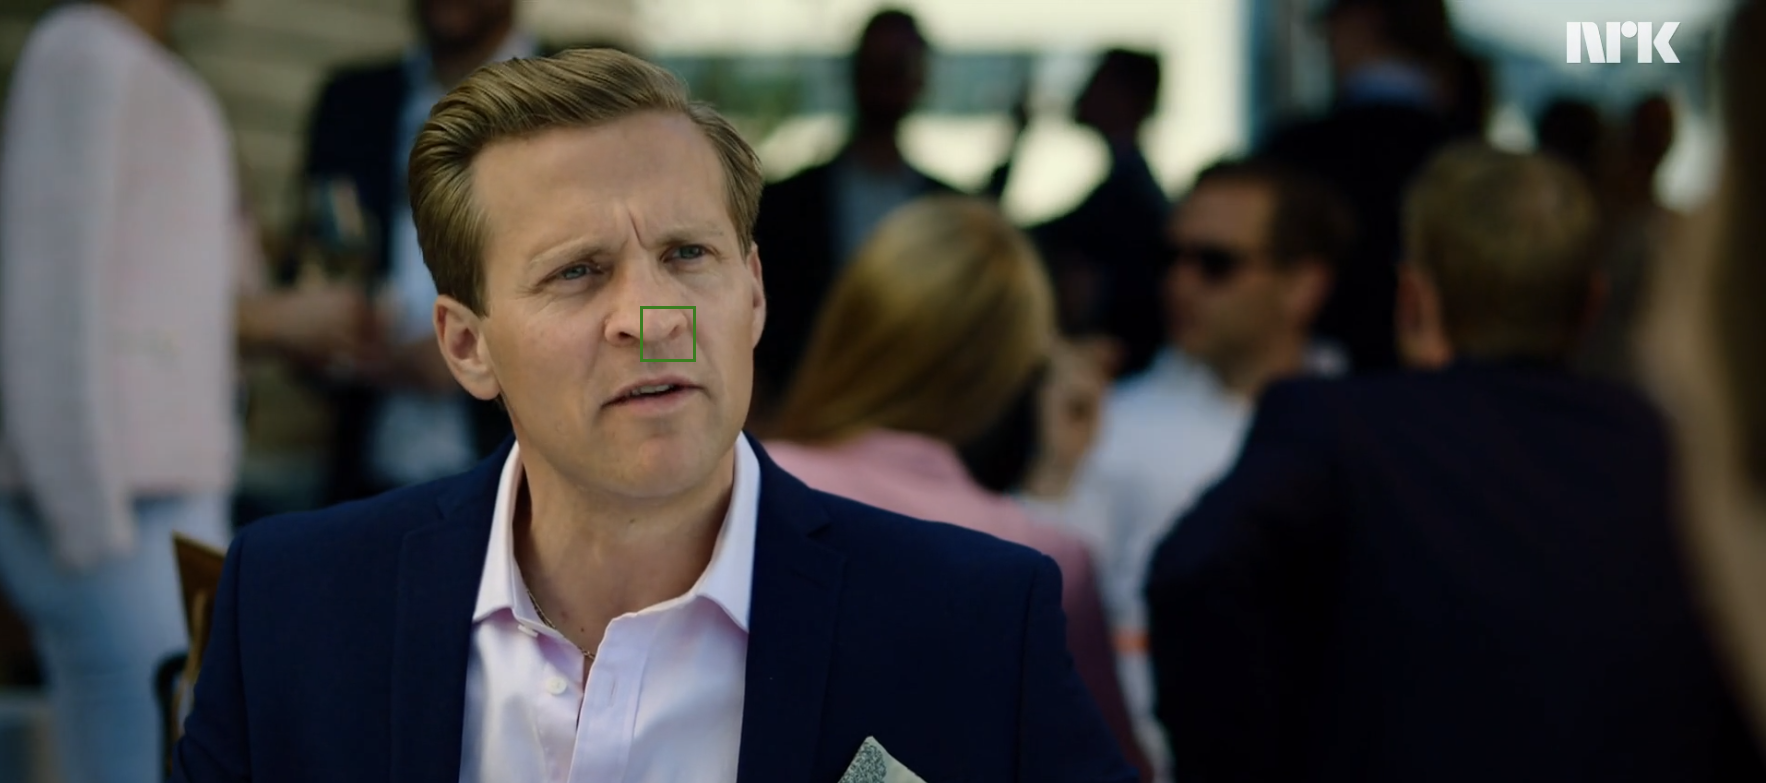
\includegraphics[width=1.0\columnwidth]{track_face.png}
\caption{AI based face tracking, the nose is selected as focus center.}
\label{fig_face_tracking}
%%\Description{A face is visible in the foreground, a blurred group in the
%% background. A box on the nose of the face shows selected focus point.}
\end{center}
\end{figure}

For scenes where there are no people, a generic image analysis model was
evaluated, providing a list of detected concepts in the image. These are then
filtered by a combination of the certainty of the observation, the size of
the object and the number of occurrences in the image. For example, a scene
with a lot of trees in it will disregard "tree".

\begin{figure}
\begin{center}
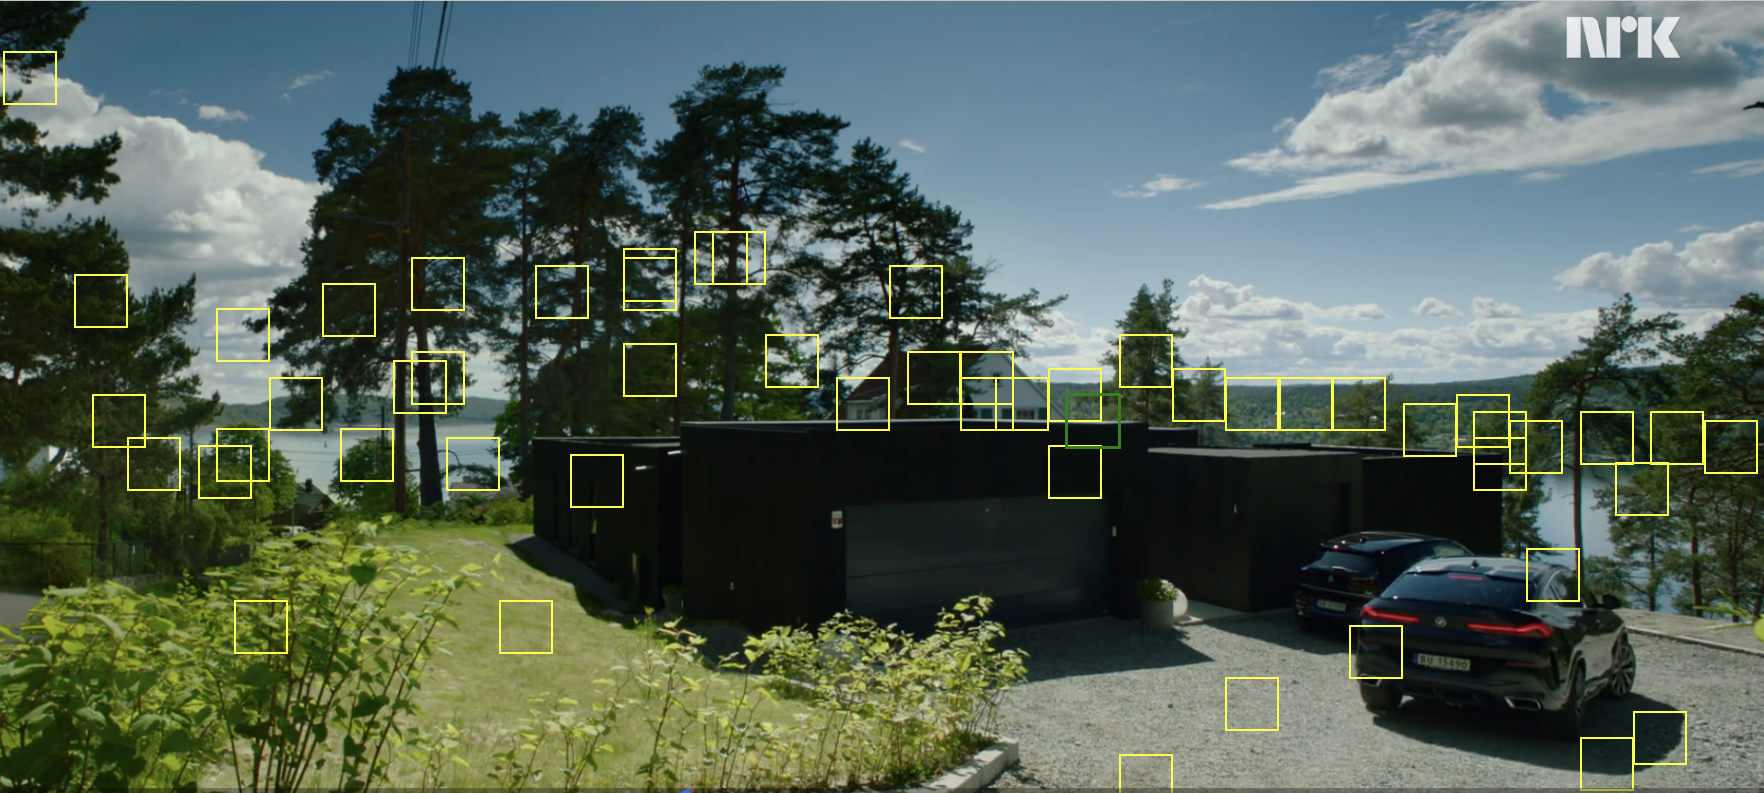
\includegraphics[width=1.0\columnwidth]{track_stuff.png}
\caption{AI detected concepts. Repeated concepts are ignored. The building is
 selected as it's largest and there is just one.}
\label{fig_stuff_tracking}
%%\Description{Image of a house surrounded by trees and two cars in front.
%% Yellow boxes show detected concepts, a green box is centered on the
%% building.}
\end{center}
\end{figure}
  
In order to test the automated process, we used three different video assets
from NRK. The first is "Valkyrien", which is an action series with a number
of fast paced scene changes, action filled scenes like car chases as well as
scenes with many people (e.g. a funeral). The second is "Vikingane"
(also available on Netflix as "Norsemen"), which is a comedy series set in
the viking era. This content has quite a few scenes with many people, where
the main characters are not prominently placed and quite a few dark scenes.
The final asset is "Exit", a "mafia" style action drama, shot with very
artistic angles. Both a manual and an automatic focus track was created for
each of the three assets. The manual tracks took a few hours to create for
each asset, as the show was watched (and parts replayed) to ensure a good
crop. The automated process was performed at approximately real-time, but no
speed optimizations were done as a part of this work.

As an alternative focus track generation method, the MediaPipe library\cite
{mediapipe} was used to provide face detections. As this returns a grid
describing features of a face, we also determine wether the face is looking
into the camera, is askew or if it's a side view. This can allow us to select
people facing the camera, or switching to a different face for a period to
simulate a more traditional multi-camera production. Using mediapipe we also
analyze every frame, which also allows us to estimate the movement of a face.
Observing debate programmes for example, the person talking is often more
mobile than those listening. This could be a good way to quickly detect the
active speaker. In this experiment, faces were sorted by their angle in
relation to the camera, then size. The more direcly people look into the
camera, the higher the rating. MediaPipe is available both in a light version
capable of running without GPU support, and a full version running on GPUs.
In this test, we used the light version for simplicity. Using the full models
on GPUs would likely provide even better results.

To test the MediaPipe approach, we used "Debatten" from NRK, which is a debate
program with a number of people, often in full figure. We created a program
that automatically downloads, analyzes and creates all necessary files
including a focus track. The process is as such fully automated given the URL
of the video. An episode of "Debatten" is about 35-45 minutes, and the
process takes about 10-15 minutes on a Lenovo laptop, including a low
resolution transcode to allow ffmpeg to detect scene shifts for more plesant
transitions on camera angle changes. Transcoding is done as I-frames are
periodic, as the video files have been optimized for streaming. If no
transcoding is possible for scene detections, other methods could be used to
detect scene changes, or these changes can be ignored and traded for the
occational flickering. 


\section{Results}

In order to validate the quality of the automated process, the AI based
positioning was compared to a manual selection where a focus point was
determined. A "hit" was defined as the crop containing the focus point, and
a "miss" as the crop not containting the focus point. This means that the
narrower the screen the higher the possibility of missing. A comparison with
a fixed crop around the center of the screen was also performed in order to
visualize the benefit of a dynamic crop. The drama series using our hybrid
face and generic AI performed very well, as illustrated in figure \ref
{generic_ai_comparison}. "Vikingane" scored worse than the other two items,
largely due to a number of scenes with a large number of people. In these
cases, the AI would often pick the wrong face. While the center crop scores
similarly as our AI on a 3:4 aspect ratio(iPad portrait), the experience is
still markedly worse as people are often placed at the edges of the screen,
making it very visible that some parts of the picture is missing.

This type of content is highly suitable for manual quality control in advance
of publishing, and it is also possible to highlight likely issues for manual
interaction. Good examples would be visually "busy" scenes without detected
faces, or if a number of people are detected over a larger area of the
screen.

\begin{figure}
\begin{center}
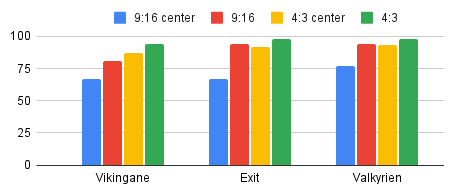
\includegraphics[width=0.7\columnwidth]{generic_ai_comparison.png}
\caption{Percentage of frames containing the focus point in drama series for DAR compared to fixed center cropping.}
\label{generic_ai_comparison}
%% \Description{Plot showing how the hit rate of the presented video is improved
%% using our method over a static centered crop.}
\end{center}
\end{figure}

For the political debate, a Pupil Labs eye tracker was used to create a
dataset of gaze information. The AI crop was then compared to the gaze data,
showing if the area watched was presented to the user. Gaze data is gathered
at 200hz and downsampled to 10hz using the median, reducing noise in the
data. We further ignored any "miss" that lasted less than 200ms, as the
person watching has to notice scene changes and possibly move the eyes to a
new position. 

\begin{figure}
\begin{center}
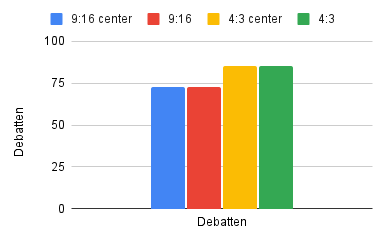
\includegraphics[width=0.7\columnwidth]{CoverageOfEyeTracking.png}
\caption{Percentage of frames containing the focus point in a debate for DAR compared to fixed center cropping.}
\label{debatten_plot}
%%\Description{Plot showing no real gain over a centered crop for Debatten.}
 \end{center}
\end{figure}

It is also important to point out that in such a debate, a number of scenes
have many people visible, making it very difficult to determine which
position is the most important. Some "misses" are therefore not really
observable by the user, if the full image is not shown. For this kind of
content, the audio is also the most important part of the experience, so
imperfections of camera angle is less critical than visually driven
experiences. Reaction shots are also often used, where the camera might
switch between a person speaking and the person expected to reply in order to
capture their body language. In figure \ref{debatten_plot} the comparison to
the eye tracking is shown.

The AI clearly has some room for improvement, as it only scores equal to a
fixed center crop. However, as illustrated in figures \ref
{debatten_both_wrong} and \ref{debatten_both_right}, the AI often provides a
more pleasing crop. The AI crop is also dynamic, and will pan automatically
to hold a person in the frame, which is particularly imporant for 9:16 crops
where a person fills most of the width. If people are looking sideways, it is
more natural to have more space in front of their face than around the back.
Our solution centers on the nose, ensuring a fairly natural crop, as shown in
figure \ref{nose_center}.

\begin{figure}
\begin{center}
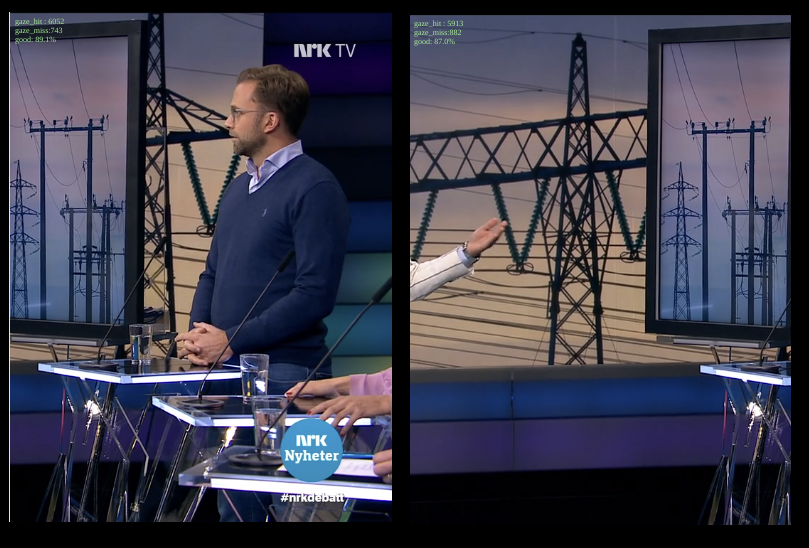
\includegraphics[width=0.8\columnwidth]{both_wrong.png}
\caption{Left crop by AI, right static center. Both are deemed "misses" as the
 eye tracker reports a different area.}
\label{debatten_both_wrong} 
%%\Description{Left crop is centered on a human, right crop has a hand sticking
%% in from the left but is otherwise just backgroud.}
\end{center}
\end{figure}

\begin{figure}
\begin{center}
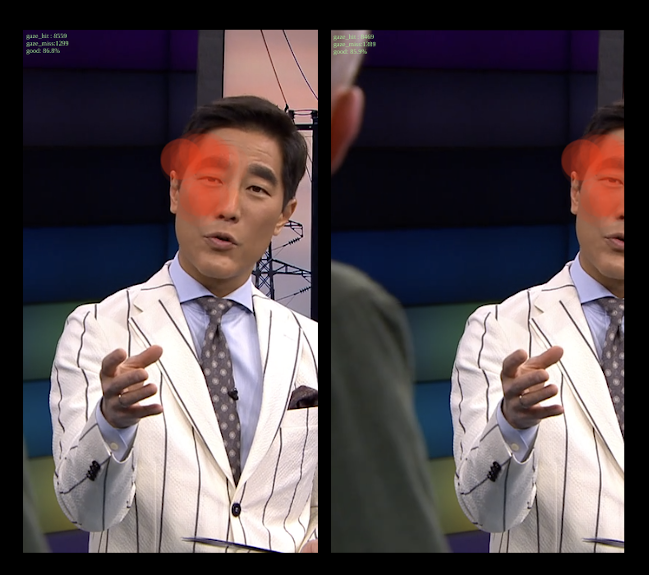
\includegraphics[width=0.8\columnwidth]{both_right.png}
\caption{Left crop by AI, right static center. Both are deemed "hits"
 according to the eye tracking data. The AI again produces as much better
 result.}
\label{debatten_both_right} 
%%\Description{Left crop is centered on a person, the right crop has the person
%% half way outside the image.}
\end{center}
\end{figure}


%%\begin{figure*}
%%\begin{center}
%%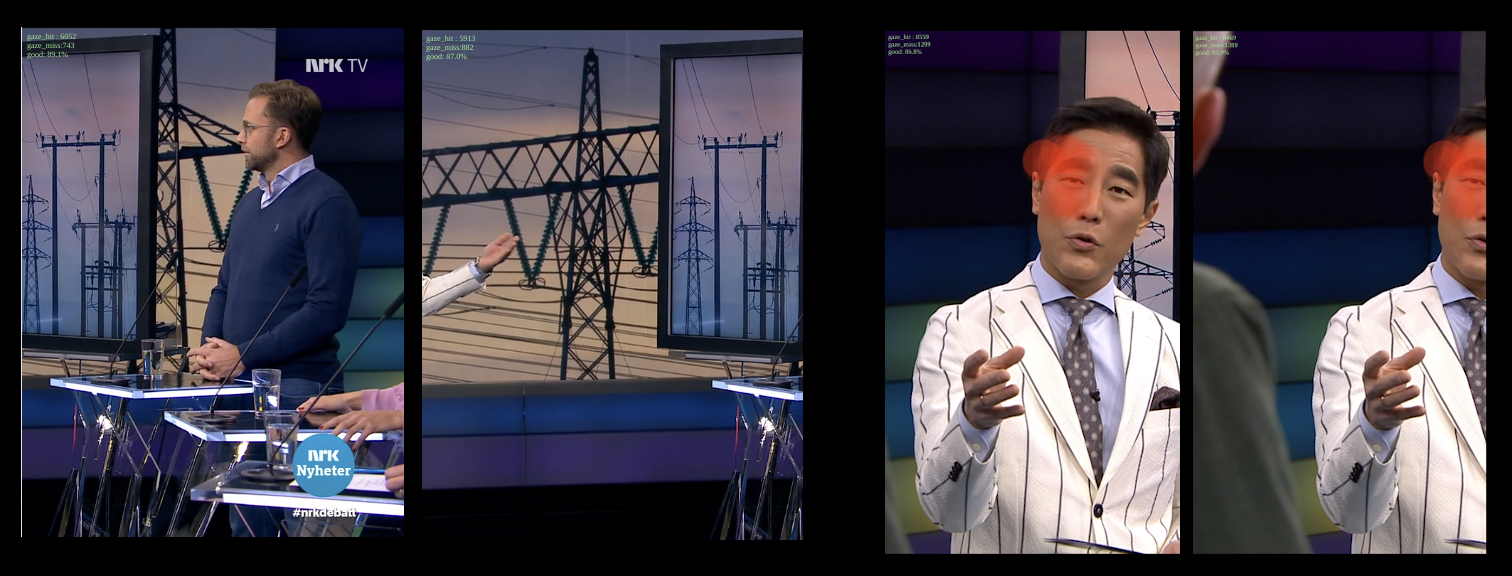
\includegraphics[width=0.7\textwidth]{debatten_both_wrong_and_right.png}
%%\caption{Two crops, the left ones are AI based, the other static center. Both 4:3 crops (left) are "misses", both 16:9 crops (right) are "hits".}
%%\label{debatten_ai_prettier} 
%%\end{center}
%%\end{figure*}

The debate was also watched in 9:16 and any suboptimal crops were noted. For
this particular episode, 7 crops were noticeably wrong, and a further 15 were
annoying (e.g. camera lingers too long on someone being interviewed), and 7
could have been better. An additional issue is with graphics embedded in the
studio, similar to weather forecast, where focus is given to the speaker, not
the image. In total, about 30 crops were imperfect in this piece of content.
The total number of focus points generated is 35.404, and ffmpeg detected 400
as scene changes. 

\begin{figure*}
\begin{center}
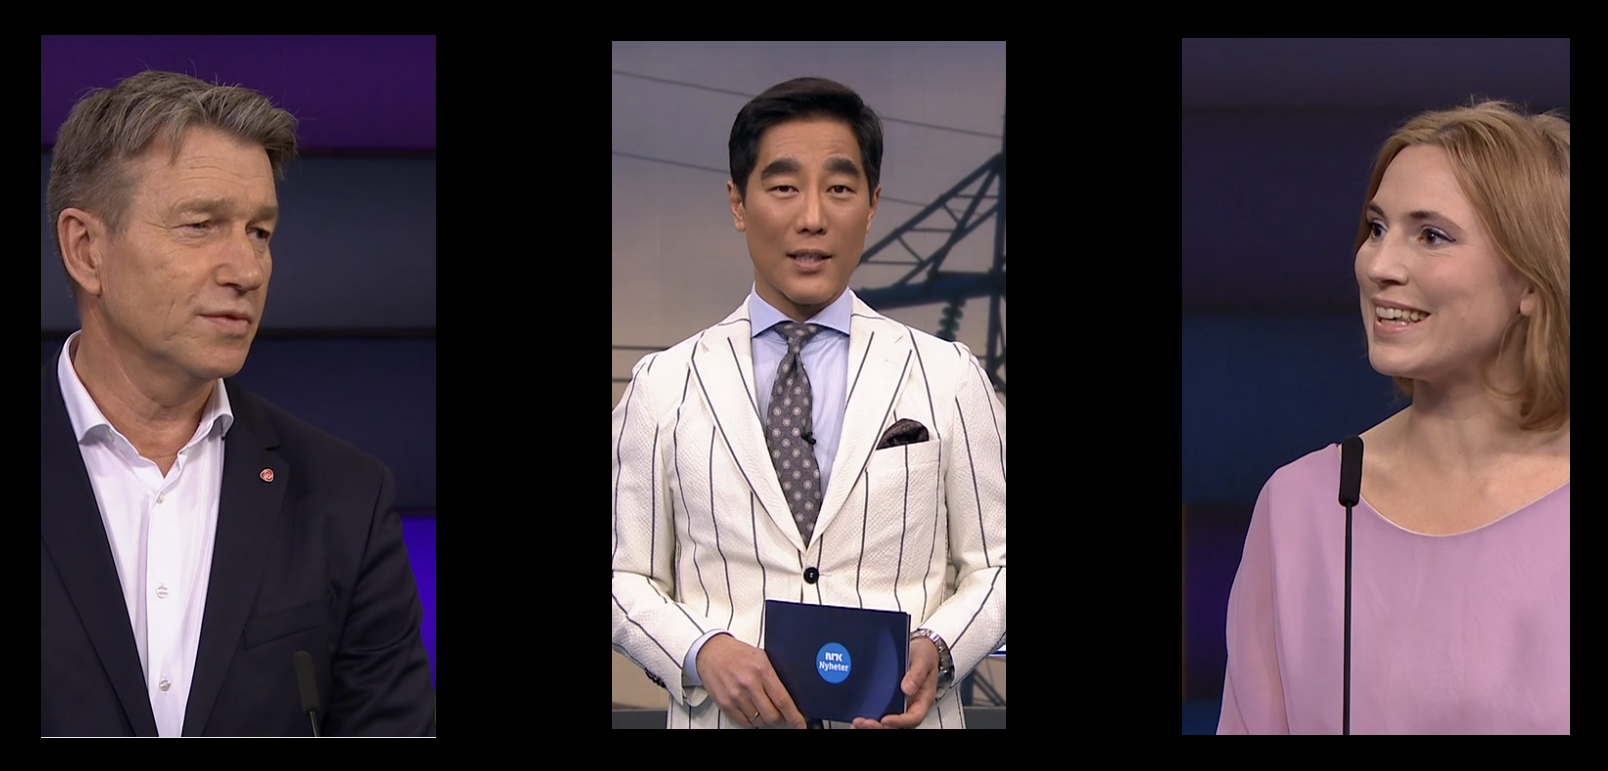
\includegraphics[width=0.9\textwidth]{nose_center.png}
\caption{Centering on the nose ensures that participants are placed naturally
 in the picture.}
\label{nose_center}
%%\Description{Three images of people. One person looks to the right and is
%% placed slightly on the left, one person is centered and looking straight
%% into the camera, the last is placed on the right and looks left. Their noses
%% are in the middle of the crop.}
\end{center}
\end{figure*}

%% TODO: The finished content were then tested by a test panel provided by <someone>, a questionnare was filled in and some panelists were interviewed. Based on the results we see <something>.


\section{Conclusions}

This paper suggests using client side video cropping to provide dynamic aspect
ratio video playback based on a focus track mapping the most important point
at any given time. Both manual positioning data and two different AI
solutions were tested. Our AI solutions worked well enough to demonstrate
feasibility even if there is room for improvement.

While larger scale user tests would be both useful and necessary for further
progress, our approach seems very promising. Allowing the clients to crop
video opens for a number of improvements to user experience. Some examples
can be rotating screens on hand held devices, allowing manual zoom levels or
ensuring overlay graphics or subtitles are placed according to likely eye
focus. This can be provided without creating multiple aspect ratio cuts of
the same content, ensuring that storage space, processing power and
complexity is limited. Dynamic aspect ratio also works perfectly with
segmented video like HLS or MPEG DASH, allowing multi-bitrate videos and
network quality adaptation to work as normal. 

The proposed solution also avoids changing production and distribution
systems, as the positioning data track is kept separate. Is is therefore
possible to retro-fit dynamic aspect ratio into any existing platform by
adding support on the client side and generating positioning tracks, for
which an automated process has also been demonstrated. This solution is also
demonstrated with a political debate, where the AI processing is performed
faster than real-time. This opens the possibility of processing the video in
parallel with online video distribution, exploiting the transmission latency
to create positioning data and send it to the clients directly. This would
allow dynamic aspect ratio to work also for live shows with no added latency
to the production or distribution.


\section{Future work}

We find the results of this early work as highly promising. Of particular
interest for future work is to incorporate custom trained AI models. Some
early experiments with a model trained on cast memebers provided some
intriguing results, but also more generic aspects like image focus, movement,
posture and repeating patterns in the video cut could be interesting to
include for a more generic solution. Including a professional producer would
also be highly beneficial in order to incorporate more knowledge of cutting,
transitions etc.


%% \bibliographystyle{plain}
\bibliography{references}
\end{document}
